\def\CommentVersion{}
\documentclass[12pt, francais, doublespacing, headsepline,oneside]{MastersDoctoralThesis}
%\usepackage[utf8]{inputenc} % Required for inputting international characters
%\usepackage[T1]{fontenc} % Output font encoding for international characters

\usepackage[utf8]{inputenc}
\usepackage[T1]{fontenc}
%\usepackage[francais]{babel}

\usepackage{palatino} % Use the Palatino font by default

\usepackage[backend=bibtex,style=authoryear,natbib=true]{biblatex} % Use the bibtex backend with the authoryear citation style (which resembles APA)

\addbibresource{mybib.bib} % The filename of the bibliography
\usepackage[autostyle=true]{csquotes} % Required to generate language-dependent quotes in the bibliography

%----------------------------------------------------------------------------------------
%	MARGIN SETTINGS
%----------------------------------------------------------------------------------------



\geometry{
	paper=a4paper, % Change to letterpaper for US letter
	inner=2.5cm, % Inner margin
	outer=2cm, % Outer margin
	bindingoffset=0cm, % Binding offset
	top=1cm, % Top margin
	bottom=1cm, % Bottom margin
	%showframe,% show how the type block is set on the page
}

%----------------------------------------------------------------------------------------
%	THESIS INFORMATION
%----------------------------------------------------------------------------------------

\thesistitle{Endormissement blabla} 
\supervisor{Dr. Abou El Hassan Benyamina \\ Dr. Houssam-Eddine ZAHAF } % Your supervisor's name,
                                          % this is used in the title
                                          % page, print it elsewhere
                                          % with \supname
\degree{Master} % Your degree name, this is used in the
                              % title page and abstract, print it
                              % elsewhere with \degreename
\author{Ismail \textsc{Yemmi}} % Your name, this is used in
                                       % the title page and abstract,
                                       % print it elsewhere
                                       % with \authorname
\addresses{50, avenue de Haley, Parce Scientifique de la haute borne, villeneuve d'ascq, 59650} 

\subject{Informatique} % Your subject area, this is not currently
                           % used anywhere in the template, print it
                           % elsewhere with \subjectname
\keywords{} % Keywords for your thesis, this is not currently used
            % anywhere in the template, print it elsewhere
            % with \keywordnames
\university{Université d'Oran 1}                                                                   % with \univname
\department{\textsc{Informatique}} % Your department's name and URL, this
                              % is used in the title page and
                              % abstract, print it elsewhere
                              % with \deptname
\grouping{\href{http://www.cristal.univ-lille.fr/emeraude/}{Emeraude}} 
\faculty{Informatique} % Your faculty's name and URL, this is used
                           % in the title page and abstract, print it
                           % elsewhere with \facname

\hypersetup{pdftitle=\ttitle} % Set the PDF's title to your title
\hypersetup{pdfauthor=\authorname} % Set the PDF's author to your name
\hypersetup{pdfkeywords=\keywordnames} % Set the PDF's keywords to
                                       % your keywords
%\usepackage[english]{babel}
%\usepackage[utf8]{inputenc}
\usepackage{listings}
\usepackage{graphicx}
\usepackage{tikz}
\usetikzlibrary{arrows,fit,shapes}
\usepackage{pgfplots}
\usepackage{algpseudocode}
\usepackage{algorithm}
\usepackage{caption}
\usepackage{minitoc}
\usepackage{multirow}
\usepackage{subcaption}
\usetikzlibrary{calc}
\usepackage{relsize}
\usepackage{url}
\usepackage{amsthm}
\usepackage{rtsched}
\tikzset{fontscale/.style = {font=\relsize{#1}}}    
\usepackage{adjustbox}
\ifdefined\CommentVersion
  \usepackage{marginnote}
  \usepackage{color}
  \usepackage{soul}
  \newcommand{\marginX}{\marginnote{\huge{\quad\quad\textbf{!}\quad\quad}}}
  \newcommand{\he}[1]{{\color{green}\marginX{}[\textbf{Houssam}: #1]}}
  \newcommand{\gl}[1]{{\color{magenta}\marginX{}[\textbf{Giuseppe}: #1]}}
  \newcommand{\ro}[1]{{\color{blue}\marginX{}[\textbf{Richard}: #1]}}
  \setstcolor{blue}
  %\newcommand{\added}[1]{{\color{blue} #1}}
  %\newcommand{\substituted}[2]{\st{#1}{\color{blue}#2}}
  %\newcommand{\deleted}[1]{\st{#1}}
\else
  \newcommand{\he}[1]{}
  \newcommand{\gl}[1]{}
  \newcommand{\ro}[1]{}
  %\newcommand{\added}[1]{{#1}}
  %\newcommand{\deleted}[1]{}
  %\newcommand{\substitute}[2]{#2}
\fi
\usepackage{capt-of}
\usepackage{mathtools}
\usepackage{amsmath,amsfonts,amssymb}
\usetikzlibrary{plotmarks}
\tikzset{
    scale plot marks/.is choice,
    scale plot marks/false/.code={
        \def\pgfuseplotmark##1{\pgftransformresetnontranslations\csname pgf@plot@mark@##1\endcsname}
    },
    scale plot marks/true/.style={},
    scale plot marks/.default=true
}
		
%%%%%%%%%%%%%%%%%%%%%%%%%%%%%%%%%%%%%%%%
%           Commandes perso            %
%%%%%%%%%%%%%%%%%%%%%%%%%%%%%%%%%%%%%%%%
\newcommand{\pow}{\mathcal{P}}
\newcommand{\pr}[1]{\mathsf{Pr}_{#1}}
\newcommand{\alp}{\texorpdfstring{\ensuremath{\upalpha}\xspace}{alpha }}
\newcommand{\alpbet}{\texorpdfstring{\ensuremath{\upalpha-\upbeta}\xspace}{alpha-b\'{e}ta}}
\newcommand{\alpt}{\ensuremath{\alpha_2}\xspace}
\newcommand{\arrival}[2]{\mathcal{A}_{#1,#2}}
\newcommand{\act}{\ensuremath{\mathsf{act}}}
\newcommand{\archi}{\mathcal{A}~}
\newcommand{\allpath}[2]{\Pi_{#1}(#2)}
\newcommand{\athr}[4]{\mathsf{aTH}_{#1,#2,#3,#4}}
\newcommand{\athrf}{\mathsf{aTH}}
\newcommand{\coeff}{\epsilon}
\newcommand{\bet}{\texorpdfstring{\ensuremath{\upbeta}\xspace}{b\'{e}ta }}
\newcommand{\bpath}[3]{\pi^{#1}_{#2}(#3)}
\newcommand{\Coef}{\ensuremath{\xi}}
\newcommand{\core}[1]{\mathsf{P}_{#1}}
\newcommand{\cutpoint}[2]{\gamma_{#1,#2}}
\newcommand{\ct}[5]{\mathsf{ct}^{#1}_{#2,#3,#4}(#5)}
\newcommand{\ctf}{\mathsf{ct}}
\newcommand{\charge}[1]{\mathsf{C}_{#1}}
\newcommand{\chargef}{\mathsf{C}}
\newcommand{\cp}{$\mathbf{CP}$}
\newcommand{\cpm}{$\mathbf{CPM}$}
\newcommand{\chargeone}[1]{\mathsf{C}_{#1}}
\newcommand{\chargeallocone}[2]{\mathsf{C}_{#1,#2}}
\newcommand{\citationchap}[2]{
	\epigraph{\og \textit{#1} \fg{}}{#2}
}
\newcommand*{\comb}[1]{{}^{#1}C_{|S_i|}}


\newcommand{\dbft}[2]{\mathsf{tdbf}({#1},{#2})}
\newcommand{\dbfts}[2]{\mathsf{dbf}({#1},{#2})}
\newcommand{\decomposition}[1]{\mathcal{D}_{#1}}
\newcommand{\deadline}[1]{\mathsf{D}_{#1}}
\newcommand{\dbf}[2]{\mathsf{dbf}(#1,#2)}
\newcommand{\dbff}{\mathsf{dbf}}
\newcommand{\dbfp}[2]{\mathsf{pdf}({#1},{#2})}
\newcommand{\dbfpf}{\mathsf{pdf}}

\newcommand{\ex}{\ensuremath{\mathsf{ex}}}
\newcommand{\excess}{\alpha}
\newcommand{\edges}[1]{\mathsf{E}_{#1}}
\newcommand{\edge}[2]{e(#1,#2)}
\newcommand{\excesstime}{\mathsf{excess\text{-}time}}

\newcommand{\freq}{\mathsf{f}}
\newcommand{\ftc}{$\mathbf{FTC}$}
\newcommand{\volt}{\mathsf{V}}
\newcommand\resp[2][]{R_#2^#1}
\newcommand{\group}[1]{\mathcal{G}_{#1}}
\newcommand{\graph}[2]{\mathsf{G}(#1,#2)}
\newcommand{\sleep}{\textsc{sleep}}
\newcommand{\job}[2]{\mathcal{J}_{#1,#2}}

\newcommand{\lookforcp}{\textbf{lookForCP}}

\newcommand{\modulo}{\%}
\newcommand{\mt}[4]{\mathsf{mt}^{#1}_{#2,#3,#4}}
\newcommand{\mtf}{\mathsf{mt}}

\newcommand{\nstrength}[1]{\Omega^{#1}}

\newcommand{\offset}[1]{\mathsf{O}_{#1}}

\newcommand{\period}[1]{\mathsf{T}_{#1}}
\newcommand{\proc}[1]{p_{#1}}
\newcommand{\random}{\mathsf{random}}

\newcommand{\strength}[1]{\mathcal{S}^{#1}}
\newcommand{\speed}[1]{\mathsf{s}_{#1}}
\newcommand{\slowest}{\ensuremath{\mathsf{sl}}}
\newcommand{\shighest}{\ensuremath{\mathsf{sh}}}
\newcommand{\soperating}{\ensuremath{\mathsf{so}}}
\newcommand{\strt}{\gls{strt}\xspace}

\newcommand{\thread}[3]{\mathsf{Th}_{#1,#2,#3}}
\newcommand{\thr}[3]{\mathsf{Th}_{#1,#2,#3}}
\newcommand{\thrftc}[2]{\mathsf{Th}_{#1,#2}}
\newcommand{\thrf}{\mathsf{Th}}
\newcommand{\taskset}[1]{\mathcal{T}_{#1}}
\newcommand{\task}[1]{\tau_{#1}}

\newcommand{\utilth}[5]{u^{#1}_{#2,#3,#4}(#5)}
\newcommand{\util}[2]{u^{#1}_{#2}}
\newcommand{\Util}[1]{U^{#1}}

\newcommand{\vertice}[2]{v_{#1,#2}}
\newcommand{\vertices}[1]{\mathsf{V}_{#1}}

\newcommand{\wcet}[5]{\mathcal{C}^{#1}_{#2,#3,#4}(#5)}
\newcommand{\wcetf}{\mathcal{C}}
\newcommand{\wcetth}[4]{\mathcal{C}^{\mathsf{th}}_{#1,#2,#3}(#4)}
%\newcommand{\wcetf}{\mathcal{C}}
\newcommand{\wcetv}[3]{\mathcal{C}^{\mathsf{v}}_{#1,#2}(#3)}
\newcommand{\wcetp}[3]{\mathcal{C}^{\mathsf{p}}_{#1}(#2)(#3)}
\newcommand{\wcetomega}[1]{\mathcal{C}^{\mathsf{\omega}}_{#1}}

\newcommand{\x}[4]{{x}_{#1,#2,#3,#4}}
\newcommand{\arrayol}{Array-OL}
\DeclarePairedDelimiter{\floor}{\lfloor}{\rfloor}
\DeclarePairedDelimiter{\ceil}{\lceil}{\rceil}
\newcommand{\citchap}[2]{
\begin{flushright}
``\textit{#1}''
\end{flushright} 
\begin{flushright}
\textbf{#2}
\end{flushright}
\minitoc
\newpage
}
	

\author{Ismail \scshape{Yemmi}}
\title{Endormissement de taches blah blah}
\begin{document}
\frontmatter % Use roman page numbering style (i, ii, iii, iv...) for
             % the pre-content pages
\pagestyle{plain} % Default to the plain heading style until the
                  % thesis style is called for the body content
\begin{titlepage}
\begin{center}
{\scshape\LARGE \univname\par}\vspace{1.5cm} % University name
\textsc{\Large }\\[0.5cm] % Thesis type
\HRule \\[0.4cm] % Horizontal line
{\huge \bfseries \ttitle\par}\vspace{0.4cm} % Thesis title
\HRule \\[1.5cm] % Horizontal line
\begin{minipage}[t]{0.4\textwidth}
\begin{flushleft} \large
\emph{Auteur:}\\
\authorname
\end{flushleft}
\end{minipage}
\begin{minipage}[t]{0.4\textwidth}
\begin{flushright} \large
\emph{Encadrants:} \\
\supname 
\end{flushright}
\end{minipage}\\[3cm]
 
\large \textit{Pour l'Obtention du Diplome \\ de \degreename~en}\\[0.3cm] 
\deptname\\[2cm] % Research group name and department name
\begin{center}
22 Juin 2017
\end{center}
%\includegraphics{Logo} % University/department logo - uncomment to place it
\begin{tabular}{llr}
\hline
\hline
Nom de Jury & Grade, Université, Belgium, Pays & Fonction \\
Nom de Jury & Grade, Université, Belgium, Pays & Fonction \\
Nom de Jury & Grade, Université, Belgium, Pays & Fonction \\
Nom de Jury & Grade, Université, Belgium, Pays & Fonction \\
\hline
\end{tabular}
\vfill
\end{center}
\end{titlepage}

\newpage
\dominitoc
\mainmatter % Begin numeric (1,2,3...) page numbering
\begin{abstract}
\addchaptertocentry{\abstractname} % Add the abstract to the table of contents


\end{abstract}


%\begingroup
%\let\cleardoublepage\clearpage
\tableofcontents
\tableofcontents
\listoffigures
\listoftables
%\endgroup


\pagestyle{thesis} % Return the page headers back to the "thesis" style

\newtheorem{mydef}{Definition}
\newtheorem{theoreme}{Theorème}    
\newtheorem{mylemma}{Lemma}     
\begin{symbols}{ll}
  % Common for all chapters
  $  \modulo $&  The rest of the ecludienne division\\
  $  \random(a,b)$& generates a random number between a and b \\
  $  \task{i}$ & Task $i$ \\  
  $  \job{i}{a}$ &  The $a^{th}$ job of task $\task{i}$\\
  $  \arrival{i}{a}$ & The arrival time of $a^{th}$ instance of task $\task{i}$ \\ 
  $  \deadline{i}$&  The relative deadline of task $\task{i}$\\
  $  \offset{i}$&  The offset of task $\task{i}$\\
  $  \period{i}$ & The period of task $\task{i}$ \\
  $  \taskset{}$& A task set  \\
  $  \taskset{j}$& The task set allocated on core $j$ \\  
  $  \archi $ &  A multicore architecture \\ 
  $  \charge{i}$ & Execution time of the single thread version of task $\task{i}$ \\ 
  $  \wcetf$& The execution time of an arbitrary thread\\
  $  \dbft{\task{i}}{t}$ & The demand bound function of task $\task{i}$ for an interval of time of length $t$  \\
  $  \dbfts{\taskset{j}}{t}$ & The demand bound function of task set $\taskset{j}$ for an interval of time of length $t$\\ 
  $  \dbff$ &  The demand bound function\\   
  $  \excess$ &  The symbol of excess time in equations \\
  $  \vec{\Coef}$ & Energy coeficients \\   
\end{symbols}

\adjustmtc
\chapter*{Introduction}
\addchaptertocentry{Introduction}

\adjustmtc
\adjustmtc
%\backmatter
\part{Partie Théorique}
\chapter{Introduction Au systeme temps réel}
\minitoc
\section{Introduction}
\section{Taxonomie sur les systèmes temps réel}
\subsection*{Différents niveaux de criticité}

Les systèmes temps réel dits critiques (ou dur) correspondent ont des
systèmes pour lesquelles il est intolérable qu’une échéance soit
manquée au risque de causer des conséquences graves, telles que des
blessures ou des pertes humaines. Les centrales nucléaires ou le
guidage de missiles représentent de tels systèmes à haute
criticité. Dans le domaine de l’informatique embarqué, l’automobile et
l’aéronautique regorgent de systèmes critiques à l’image des
équipements déclencheurs d’airbags ou des logiciels de contrôle de vol
de satellite. Il est crucial que les résultats soient disponibles au
moment voulu et un résultat obtenu trop tard est inutilisable, à
l’instar d’un système anti-missile qui recevrait la position d’un
objet volant avec du retard.

Les systèmes temps réels mou sont des systèmes où on tolère les
retards et ne requièrent pas un déterminisme temporel aussi fort que
les systèmes temps réels dur.  Par exemple, un logiciel de diffusion
de flux vidéo produit un certain nombre d’images dans un intervalle de
temps régulier. Le fait de manquer une ou plusieurs échéances ne
provoque pas l’arrêt du système multimédia. La qualité de la vidéo est
dégradée mais le service peut continuer de fonctionner sans
risque. Donc les systèmes temps réels mou offre le meilleur service
possible (notion de best effort) et les retards dans l’obtention des
résultats ne sont pas dramatiques.

A la frontière entre les systèmes temps réel dur et mou, les systèmes
temps réel ferme tolèrent une certaine proportion d’échéances
manquées. Ils ne considèrent que les résultats obtenus à temps et sont
liés à la notion de qualité de service (QoS).

\section{Modélisation des tâches}
Liu et Layland \cite{LL73} ont proposé une modelisation d'un systemes
temps réel Soit un système temps réel composé d’un ensemble de tâches
nommé $\taskset{}$ qui comprend n tâches périodiques dont les
caractéristiques sont détaillées ci-dessous. Nous définissons dans
cette section tous les termes qui seront utilisés en relation avec la
notion d’ensemble de tâches.
\begin{description}
\item[Tâche :] Une tâche $\task{}$ est définie comme l’exécution
  d’une suite d’instructions. Nous supposons que toutes les tâches
  sont indépendantes et que l’ordre dans lequel les tâches sont
  exécutées n’a pas de conséquence sur la bonne exécution du système
  du moment qu’elles respectent leurs contraintes temporelles. Nous
  faisons également l’hypothèse que les tâches sont synchrones, donc
  que toutes les tâches sont actives dès que le système débute son
  exécution, les tâches sont toutes libérées simultanément. Le modèle
  de tâches que nous utilisons est le modèle de tâches dit périodique
  pour l’ordonnancement fixe et sporadique pour l’ordonnancement
  dynamique.
\item[Travail (Job) :] Chaque tâche libère périodiquement des
  travaux. Un travail est une suite d’instructions qui doit être
  réalisée avant une date fixée. Lorsqu’une tâche libère un travail,
  celui-ci est prêt à être exécuté et devient disponible pour
  l’algorithme d’ordonnancement. Une tâche $\task{i}$ libère ses travaux
  périodiquement suivant sa période Ti, un travail n’a donc pas de
  période associée. Ce modèle est appelé modèle de tâche périodique
  car chaque travail est libéré exactement lorsque la tâche atteint sa
  période. D’autres modélisations plus souples existent comme les
  systèmes de tâches sporadiques ou apériodiques. Pour les systèmes
  sporadiques, la période d’une tâche est la période de temps minimale
  entre deux libérations de travaux pour une tâche, ce qui signifie
  que le système ne peut savoir la date exacte où le travail va être
  libéré. Dans le cas de systèmes apériodiques, l’intervalle de temps
  entre deux libérations de travaux n’est soumis à aucune
  contrainte. Ces systèmes sont plus difficiles à étudier du fait de
  l’imprévisibilité de l’arrivée des tâches.
\item[Hyperpériode :] L’hyperpériode H de l’ensemble de tâches
  correspond au plus petit commun multiple de toutes les périodes de
  l’ensemble de tâches.  $H =
  PPCM(\{\period{0},\period{1},\cdots,\period{n}\})$ Le nombre de
  tâches dans un système temps réel embarqué est limité et les
  périodes de ces tâches ont en général des relations temporelles
  entre elles. Par exemple, il est peu probable que les périodes des
  tâches soient premières entre elles, les périodes des tâches sont
  souvent des harmoniques. En prenant un exemple concret, des tâches
  peuvent avoir des périodes de 1ms, 2ms, 5ms ou 10ms mais il est
  moins fréquent de trouver des tâches avec des périodes de 1.78ms et
  de 8.54ms. La valeur de l’hyperpériode ainsi que le nombre de
  travaux dans une hyperpériode restent donc naturellement
  raisonnables.
\item[Date Réveil :] notée $r_i$, c’est la date où la tache libère
  son premier travail, chaque travail de la tâche est libéré à
  l’instant $r_{i} + K\period{i}~avec~K \in \mathbb{N}$
\item[Pire temps d’execution (Worst Case Execution Time WCET) :] est
  la durée maximale de l’exécution de chacun de ses travaux. Le WCET
  de la tâche $\task{i}$ est noté Ci. Calculer le WCET d’une tâche est
  difficile et ce sujet est une thématique de recherche à lui tout
  seul. Nous renvoyons le lecteur à \cite{WEE+08} pour plus
  d’informations. Nous supposons que le WCET de chaque travail est
  connu.
\item[Échéance(Deadline):] Chaque travail une fois libéré doit
  terminer son exécution avec une certaine date sous peine de violer
  son échéance. Nous notons
  Di l’échéance relative de la tâche

  $\task{i}$. L’échéance absolue $j.d$ du travail $j$ sera donc la
  date de sa libération additionnée de cette échéance relative.

Il existe trois types de modèles  de taches : 

\begin{itemize}
\item Modèles à « échéances implicites » où l’échéance de
  chaque travail égale à sa période $\period{i} = \deadline{i}$.
\item Modèles à « échéances contraintes » où l’échéance de
  chaque travail est inférieure ou égale à sa période $\deadline{i} <=
  \period{i}$.
\item le modèle à «échéances arbitraires» ne fixe aucune
  contrainte entre les échéances et les périodes des tâches.
\end{itemize}

\item[Utilisation d’une tâche :] L’utilisation d’une tâche est le
  rapport entre son WCET et sa période. L’utilisation $U_i$ de la
  t\^ache $\task{i}$ est donc
  $\frac{\charge{i}}{\period{i}}$
\item[Utilisation globale de l’ensemble de tâches :] L’utilisation
  globale U de l’ensemble de tâches est la somme de toutes les
  utilisations individuelles des tâches de l’ensemble de tâches :

\begin{equation}
U = \sum_{i=1}^n U_i
\end{equation}

\end{description}

\section{Ordonnancement monoprocesseur}
Un algorithme d’ordonnancement monoprocesseur est chargé
de répartir les tâches sur un processeur : il décide quelle tâche sera
exécutée sur le processeur et pour combien de temps.
\subsection*{Definition}
Nous définissons dans un premier temps les termes
habituels concernant les systèmes temps réel : \\
\begin{description}
\item[Hors-ligne / en-ligne:] Un algorithme d’ordonnancement
  hors-ligne prend la totalité de ses décisions d’ordonnancement avant
  l’exécution du système. Au contraire, un ordonnancement en-ligne
  prend les décisions d’ordonnancement lors de l’exécution
\item[Priorités:] Les algorithmes d’ordonnancement temps réel peuvent
  être classés suivant leur utilisation des priorités pour choisir
  quelle tâche doit être ordonnancée.
\item[Préemptif / non préemptif:] Un algorithme d’ordonnancement
  préemptif est un algorithme d’ordonnancement qui peut arrêter
  l’exécution d’une tâche, i.e. la préempter, à tout moment lors de
  l’exécution. Au contraire, un algorithme d’ordonnancement non
  préemptif ne permet aucune préemption, un travail en cours
  d’exécution ne peut être arrêté.
\item[Ordonnançabilité / Faisabilité:] Un système de tâches est dit
  ordonnançable si un ordonnancement existe permettant de satisfaire
  toutes les contraintes temps réel. Un système de tâches est dit
  faisable s’il existe un algorithme d’ordonnancement permettant
  d’ordonnancer ce système de tâches sans aucune violation
  d’échéances.
\item[Optimalité:] Un algorithme d’ordonnancement est dit optimal s’il
  peut ordonnancer tous les ensembles de tâches ordonnançables par
  d’autres algorithmes d’ordonnancement existants.
\end{description}
\subsection{Algorithme d’ordonnancement à priorité fixe}
\subsubsection{Rate Monotonic \cite{LL73}}
Rate Monotonic est un algorithme à priorité fixe
introduit par Liu et Layland dans \cite{LL73}. Cet algorithme affecte
des priorités aux tâches inversement proportionnel à leur période :
plus leur période est petite, plus la tâche est prioritaire.

Un exemple de système de tâche ordonnancée par Rate
Monotonic est donné table \ref{tab:exempleRM}. La figure
\ref{fig:exempleRM} est une représentation graphique de
l'ordonnancement correspondant.

\begin{table}[h]
\begin{center}
\begin{tabular}{|c|c|c|c|}
 \hline $\task{i}$ & $\charge{i}$ & $\period{i}$ & priorité\\ 
 \hline 1 & 1 & 10 & 3\\ 
 \hline 2 & 1 & 4 & 0\\ 
 \hline 3 & 1 & 5 & 1\\ 
 \hline 4 & 2 & 8 & 2\\ 
 \hline
 \end{tabular}
\end{center}
\caption{ensemble de tache avec priorité affecté par Rate Monotonic} \label{tab:exempleRM}
\end{table}

%\begin{figure}[h]
%\begin{center}
%\begin{RTGrid}[height=4cm, width=12cm, labelsize=8pt, numbersize=6]{4}{13}
%  \multido{\n=0+4}{3}{
%    \TaskArrDead{2}{\n}{4}}
%  \TaskExecution{2}{0}{1}
%  \TaskExecution{2}{4}{5}
%  \TaskExecution{2}{8}{9}
%  \TaskExecution{2}{12}{13}
%  \multido{\n=0+5}{2}{
%    \TaskArrDead{3}{\n}{5}}
%  \TaskExecution{3}{1}{2}
%  \TaskExecution{3}{5}{6}
%  \TaskExecution{3}{10}{11}
%  \multido{\n=0+8}{1}{
%    \TaskArrDead{4}{\n}{8}}
%  \TaskExecution{4}{2}{4}
%  \TaskExecution{4}{9}{10}
%  \TaskExecution{4}{11}{12}
%  \multido{\n=0+10}{1}{
%    \TaskArrDead{1}{\n}{10}}
%  \TaskExecution{1}{6}{7}
%\end{RTGrid}
%\caption{Ordonnancement sous Rate Monotonic} \label{fig:exempleRM}
%\end{center}
%\end{figure}

\begin{theoreme}
Rate Monotonic est optimal pour l'ordonnancement de systèmes de tâches
synchrones, indépendantes et à échéance sur requête en présence de
préemption.
\end{theoreme}

\begin{theoreme}[Condition Suffisante \cite{LL73}].
  Un système temps réel composé de n tâches est ordonnançable par Rate
  Monotonic si :
\begin{equation}
U = \sum_{i=1}^n \frac{\charge{i}}{\period{i}} \leq n ( 2^{\frac{1}{n}}
- 1)
\end{equation}
\end{theoreme}

\subsubsection{Deadline Monotonic \cite{LW82}}
Deadline Monotonic est un algorithme à priorité fixe
introduit par Leung et Whitehead dans \cite{LW82}.

Cet algorithme est proche de celui de Rate Monotonic, à la différence
que les priorités sont maintenant affectées en fonction de l'échéance
relative de chaque tâche au lieu de leur période.

\begin{theoreme}
Cet algorithme est optimal dans le cadre des algorithmes à priorité
fixe pour des systèmes de tâches synchrones à échéance contrainte
lorsque la préemption est autorisée. Monotonic et Deadline Monotonic
se confondent.
\end{theoreme}

\textbf{Condition suffisante d'ordonnançabilité} La condition
suffisante d'ordonnançabilité est inspirée de la condition suffisante
d'ordonnançabilité de Liu et Layland (cf. théorème 4) :

\begin{theoreme}
 Un système temps réel composé de n tâches est ordonnançable par Deadline
Monotonic si la condition suivante est vérifiée :
\begin{equation}
U = \sum_{i=1}^n \frac{\charge{i}}{\deadline{i}} \leq n ( 2^{\frac{1}{n}} - 1)
\end{equation}
\end{theoreme}

\textbf{Condition necessaire et suffisante d'ordonnançabilité} Joseph
et al. \cite{JP86} ont proposé un test d’ordonnancabilité basé sur le
pire temps de reponse $R_{i}$.  Le pire temps de réponse est le moment
ou la tache $i$ de priorité $p$ terminera son exécution quand les
taches les plus prioritaire sont actifs avec elle en même temps.\\

\begin{theoreme}
soit $\taskset{}$ = \{ $\task{1},\task{2},\cdots, \task{n} \}$ un ensemble de $n$
taches.  $\taskset{}$ est ordonnancable sous deadline monotonic si et seulement si:
\begin{equation}
\forall \task{i} \in \taskset / R_{i} \leq \deadline{i}
\end{equation}

%\begin{equation}
%R_{i} = \left\lbrace
%\begin{array}{l}
%R_{i}^0=\wcet{i}
%\\
% R_{i}^{(k+1)}=\charge{i}+\sum_{j \in pr(i)}  \left \lceil 
% \frac{R_{i}^{(k)}}{\period{j}} \right \rceil * \wcet{j}  
%\end{array}
%\right.
%\end{equation}
\end{theoreme}

\begin{table}[h]
\begin{center}
\begin{tabular}{|c|c|c|c|c|c|}
 \hline$\task{i}$ & $\charge{i}$ & $\deadline{i}$ & $\period{i}$ & $\pr{i}$ & $R_i$\\ 
 \hline1 & 1 & 5 & 10 & 2 & 3\\ 
 \hline2 & 1 & 3 & 4 & 0 & 1\\ 
 \hline3 & 1 & 4 & 5 & 1 & 2\\ 
 \hline4 & 2 & 7 & 8 & 3 & 7\\ 
 \hline
 \end{tabular}
\end{center}
\caption{ensemble de tache avec priorité affecté par Deadline
  Monotonic} \label{tab:exempleDM}
\end{table}


%\begin{figure}[h]
%\begin{center}
%\begin{RTGrid}[height=4cm,width=12cm,labelsize=8pt,numbersize=6]{4}{10}
%\multido{\n=0+10}{1}{
%\TaskArrDead{1}{\n}{5}}
%\TaskExecution{1}{2}{3}

%\multido{\n=0+4}{2}{
%\TaskArrDead{2}{\n}{3}}
%\TaskExecution{2}{0}{1}
%\TaskExecution{2}{4}{5}
%\TaskExecution{2}{8}{9}

%\multido{\n=0+5}{2}{
%\TaskArrDead{3}{\n}{4}}
%\TaskExecution{3}{1}{2}
%\TaskExecution{3}{5}{6}

%\multido{\n=0+8}{1}{
%\TaskArrDead{4}{\n}{7}}
%\TaskExecution{4}{3}{4}
%\TaskExecution{4}{6}{7}
%\end{RTGrid}
%\caption{Ordonnancement sous Deadline Monotonic} \label{fig:exempleDM}
%\end{center}
%\end{figure}


\subsection{Algorithme d’ordonnancement à priorité dynamique}
Les algorithmes à priorité dynamique affectent une priorité qui n'est
plus une donnée statique.  La priorité d'une tâche est mise à jour
durant la vie du système en fonction de certains critères, les
critères utilisés dépendant de l'algorithme utilisé.

\subsubsection{Earliest Deadline First\cite{LL73}}
Earliest Deadline First est un algorithme connu et étudié depuis
longtemps \cite{LL73, Der74, Hor74}. Le principe de cet algorithme est
d'accorder la priorité la plus grande à la tâche ayant une instance
dont l'échéance absolue est la plus proche.  L'avantage majeur de cet
algorithme est qu'en présence d'un système de tâche à échéance sur
requête, le taux d'utilisation maximum du processeur est de 100\%
(théorème 8).

\begin{theoreme}[\cite{LL73}]
 Un système de n tâches à échéance contrainte est ordonnançable par
 Earliest Deadline First si et seulement si :
 \begin{equation}
 U \leq 1
 \end{equation}
\end{theoreme}

\paragraph{Fonction de demande du processeur}

La demande du processeur des tâches devant se terminer avant la date t
(c’est-à-dire dont l’échéance est avant ou à la date t), notée
dbf($\taskset{}$, t) (Demand Bound Function) est définie par la durée
cumulée des requêtes dont la date d’activation et l’échéance sont dans
l’intervalle de temps[0, t]:

\begin{equation}
DBF(\taskset{},t) = \sum_{\task{} \in \taskset{}}dbf(\task{},t)
\end{equation}
%
%\begin{equation}
%dbf(\task{},t) = max \bigg( 0,\bigg( \bigg\lfloor \frac{t - \deadline{i}}{\period{i}} \bigg\rfloor + 1 \bigg) \times \wcet{i} \bigg)
%\end{equation}

\paragraph{Condition necessaire et suffisante
  d'ordonnançabilité}\cite{BHR93} il existe un test d’ordonnancabilité
basée sur la fonction de la demande processeur DBF($\taskset,t$)
causée par des tâches activées et devant être terminées dans
l’intervalle [0, t].

\begin{theoreme}
Un système $\taskset{}$ de $n$ tâches à échéance contrainte est
ordonnançable par Earliest Deadline First si et seulement si :
\begin{equation}
\forall t \geq 0 , DBF(\taskset,t) \leq t 
\end{equation}
\end{theoreme}

\begin{theoreme}[\cite{Der74}]
Earliest Deadline First est optimal pour ordonnancer des systèmes de
tâches indépendantes lorsque le facteur d'utilisation U du système est
inférieur ou égale à 1 (absence de surcharge).
\end{theoreme}

\begin{table}[h]
\begin{center}
\begin{tabular}{|c|c|c|c|}
 \hline$\task{i}$ & $\charge{i}$ & $\deadline{i}$ & $\period{i}$\\ 
 \hline1 & 3 & 4 & 5\\ 
 \hline2 & 3 & 7 & 7 \\  
 \hline
 \end{tabular}
\end{center}
\caption{ensemble de tache } \label{tab:exempleEDF}
\end{table}


%\begin{figure}[h]
%\begin{center}
%\begin{RTGrid}[height=4cm,width=12cm,labelsize=8pt,numbersize=6]{2}{16}
%\multido{\n=0+5}{3}{
%\TaskArrDead{1}{\n}{4}}
%\TaskExecution{1}{0}{3}
%\TaskExecution{1}{6}{9}
%\TaskExecution{1}{12}{15}


%\multido{\n=0+7}{2}{
%\TaskArrDead{2}{\n}{7}}
%\TaskExecution{2}{3}{6}
%\TaskExecution{2}{9}{12}


%\end{RTGrid}
%\caption{Ordonnancement sous EDF} \label{fig:exempleEDF}
%\end{center}
%\end{figure}

\section{Ordonnancement Multiprocesseur}
L'ordonnancement multiprocesseur se distingue de l'ordonnancement
monoprocesseur par la présence de plusieurs processeurs sur lesquels
peuvent s'exécuter les tâches. Se pose alors certains problèmes parmis
eux :
\begin{itemize}
\item[$\bullet$] le problème de placement des tâches : sur quel(s) processeur(s) une tâche va-t-elle s'exécuter ?
\item[$\bullet$] le problème de la migration des tâches : une tâche peut-elle changer de processeur pour s'exécuter ?
\item[$\bullet$] le problème de l'ordonnancement des tâches : affectation des priorités.
\end{itemize}

Nous allons nous intéressé uniquement au problème de placement et
d'ordonnancement des tâches, sans prendre en compte la migration et
nous supposerons que les tâches sont indépendantes.

\subsection{Classification}
 Les algorithmes d'ordonnancement peuvent être classés
dans différentes catégories, en fonction de leurs caractéristiques :
\begin{itemize}
\item  stratégie globale : sur un système comprenant m
  processeurs, un algorithme d'ordonnancement utilisant une stratégie
  globale va affecter les m tâches les plus prioritaires aux m
  processeurs.
\item  stratégie partitionner : le principe d'un algorithme
  utilisant une stratégie par partitionnement est de placer chaque
  tâche sur un processeur, et ensuite d'exécuter sur chaque processeur
  un algorithme d'ordonnancement monoprocesseur.
\item stratégie par semi partitionner : Elle est obtenue
  par combinaison de la stratégie par partitionnement et de la
  stratégie globale.
\end{itemize}
Il est à noter qu'il n'y a pas une catégorie qui soit
meilleure qu'une autre. Il existe des systèmes de tâches qui peuvent
être ordonnancés en utilisant une stratégie globale mais pas avec une
stratégie par partitionnement et inversement. On dit que ces
algorithmes sont non comparables \cite{LW82}.

\subsection{Optimalité}
\begin{theoreme}[\cite{HL92}]
Il n'existe pas d'algorithme en-ligne optimal pour des systèmes
multiprocesseurs. Toutefois, lorsqu'on restreint le cadre d'étude et
que l'on ne considère uniquement des systèmes de tâches périodiques,
alors il existe des algorithmes optimaux, comme les algorithmes de
type Pfair par exemple.
\end{theoreme}

\subsection{Algorithme d'ordonnancement utilisant une stratégie par partitionnement}
\subsubsection{Généralité}
Les algorithmes utilisant une stratégie par
partitionnement relèvent dans la plupart des cas du problème du
bin-packing, c'est-à-dire comment trouver un placement pour l'ensemble
des tâches sur un nombre minimum de processeurs.  Ce problème de
partitionnement des tâches pour les placer sur les processeurs a été
montré comme étant NP-difficile dans \cite{LW82}. Il n'existe donc pas
d'algorithmes s'exécutant en temps polynomial permettant de trouver
une solution optimale à ce problème. Toutefois, il existe des
heuristiques permettant d'obtenir des résultats corrects en temps
polynomial.
\subsubsection{First-Fit et Best-Fit}
Parmi les heuristiques existantes pour résoudre ce type de problème,
il existe quatre heuristiques First Fit, Best Fit, Next Fit et Worst
Fit qui reposent tous sur le même principe : on affecte chaque tâche
dans l'ordre à un processeur, selon un critère d'acceptation.  La
différence entre les deux types d'algorithmes réside sur la manière
dont est placée chaque tâche :
\begin{itemize}
\item[$\bullet$] First Fit : la tâche est placée sur le premier
  processeur avec un ensemble de tache ordonnançable ;
\item[$\bullet$] Next Fit : même principe que First Fit ...
\item[$\bullet$] Best Fit : la tâche est placée sur le processeur avec
  un ensemble de tache ordonnançable et ayant le taux d'utilisation
  maximal.
\item[$\bullet$] Worst Fit : la tâche est placée sur le processeur
  avec un ensemble de tache ordonnançable et ayant le taux
  d'utilisation minimal.
\end{itemize}
Les algorithmes de type First Fit ou Best Fit ne sont pas les seuls
existants il existe aussi Next Fit ou aussi Worst Fit.

La table \ref{tab:exampleFFBF} et les figures \ref{fig:exemplFF} et
\ref{fig:exemplBF} illustre les deux heuristiques de placement
First-Fit et Best-Fit sur un ensemble de 10 taches periodiques et 4
processeurs.

\begin{table}[!h]
\begin{center}
\begin{tabular}{|c|c|c|c|}
 \hline$\task{i}$ & $\charge{i}$ & $\deadline{i}$ & $\period{i}$ \\ 
 \hline1 & 5 & 10 & 10 \\ 
 \hline 2 & 7 & 21 & 21 \\ 
 \hline 3 & 3 & 22 & 22 \\ 
 \hline 4 & 1 & 24 & 24 \\ 
 \hline 5 & 10 & 30 & 30 \\ 
 \hline 6 & 16 & 40 & 40 \\ 
 \hline 7 & 1 & 50 & 50 \\ 
 \hline 8 & 3 & 55 & 55 \\ 
 \hline 9 & 9 & 70 & 70 \\ 
 \hline 10 & 17 & 100 & 100 \\ 
 \hline 
 \end{tabular}
\end{center}
\caption{Ensemble de taches periodiques} \label{tab:exampleFFBF}
\end{table}

\begin{figure}[!h]
\begin{center}
\begin{tikzpicture}
%\draw (0,0) rectangle (1.5,1);
\node at (-0.5,0.5) {P4};
\node at (-0.5,1.5) {P3};
\node at (-0.5,2.5) {P2};
\node at (-0.5,3.5) {P1};
\draw (0,1) rectangle (1.5,2) node[pos=.5] {$\task{6}$};
\draw (0,2) rectangle (1.5,3) node[pos=.5] {$\task{2}$};
\draw (0,3) rectangle (1.5,4) node[pos=.5] {$\task{1}$};
\draw (1.5,1) rectangle (3,2) node[pos=.5] {$\task{9}$};
\draw (1.5,2) rectangle (3,3) node[pos=.5] {$\task{5}$};
\draw (1.5,3) rectangle (3,4) node[pos=.5] {$\task{3}$};
\draw (3,1) rectangle (4.5,2) node[pos=.5] {$\task{10}$};
\draw (3,3) rectangle (4.5,4) node[pos=.5] {$\task{4}$};
\draw (4.5,3) rectangle (6,4) node[pos=.5] {$\task{7}$};
\draw (6,3) rectangle (7.5,4) node[pos=.5] {$\task{8}$};
\draw (0,0) rectangle (7.5,4);
\draw (0,0) rectangle (7.5,4);
\draw (0,0) rectangle (7.5,3);
\draw (0,0) rectangle (7.5,2);
\draw (0,0) rectangle (7.5,1) node[pos=.5] {$\emptyset$};
\end{tikzpicture}
\caption{Placement de taches en First Fit par les contraintes
  DM} \label{fig:exempleFF}
\end{center}
\end{figure}

\begin{figure}[!h]
\begin{center}
\begin{tikzpicture}
\node at (-0.5,0.5) {P4};
\node at (-0.5,1.5) {P3};
\node at (-0.5,2.5) {P2};
\node at (-0.5,3.5) {P1};
\draw (0,0) rectangle (1.5,1) node[pos=.5] {$\task{4}$};
\draw (0,1) rectangle (1.5,2) node[pos=.5] {$\task{3}$};
\draw (0,2) rectangle (1.5,3) node[pos=.5] {$\task{2}$};
\draw (0,3) rectangle (1.5,4) node[pos=.5] {$\task{1}$};

\draw (1.5,0) rectangle (3,1) node[pos=.5] {$\task{5}$};
\draw (1.5,1) rectangle (3,2) node[pos=.5] {$\task{6}$};
\draw (1.5,2) rectangle (3,3) node[pos=.5] {$\task{7}$};

\draw (3,0) rectangle (4.5,1) node[pos=.5] {$\task{9}$};
\draw (3,2) rectangle (4.5,3) node[pos=.5] {$\task{8}$};

\draw (4.5,0) rectangle (6,1) node[pos=.5] {$\task{10}$};
\draw (0,0) rectangle (7.5,4);
\draw (0,0) rectangle (7.5,4);
\draw (0,0) rectangle (7.5,3);
\draw (0,0) rectangle (7.5,2);
\draw (0,0) rectangle (7.5,1);
\end{tikzpicture}
\caption{Placement de taches en Best Fit par les contraintes
  DM} \label{fig:exempleBF}
\end{center}
\end{figure}
\section{Conclusion}

\chapter{Etat de l'art}
\minitoc
\section{Introduction}
\section{Les modèles de consommation d'énergie DVFS et DPM}
L’énergie consommée par un processeur est l'integrale de
la puissance dissipée et du temps d’exécution. Nous utiliserons
principalement la notion de consommation énergétique et non de
puissance. Cette consommation énergétique est divisée en consommation
statique et consommation dynamique. Nous détaillons dans cette section
les modèles des consommations dynamique et statique et montrons que la
consommation statique est récemment devenue plus importante que la
consommation dynamique.
\subsection{Consommation dynamique}

Mei et al.\cite{Mei13}, ont défini la dissipation de puissance
dynamique par un circuit CMOS comme produit de Un coefficient constant
qui dépend de la technologie utilisée pour fabriquer la puce, par la
Carré de la tension et par la fréquence.
\begin{equation}
\pow_{dynamique} = \coeff * \freq * \volt^2 
\end{equation}
Où $\coeff$ correspond à la capacité de sortie du circuit et $\volt$ à
la tension d’alimentation.

Les solutions permettant de réduire la puissance dynamique dans les
circuits s’attachent par conséquent à réduire la fréquence de
fonctionnement. La relation précédente montre qu’il est moins
économique d’un point de vue énergétique de faire fonctionner un
circuit à pleine vitesse que de faire fonctionner un circuit à vitesse
réduite pendant un laps de temps plus important.

La technique permettant de réduire la vitesse du système est appelée
DVFS (Dynamic Voltage and Frequency Scaling) et tire parti du fait que
les processeurs ont plusieurs fréquences et plusieurs tensions de
fonctionnement. De nombreux algorithmes d’ordonnancement ont été
proposés utilisant cette solution \cite{WWDS94, YDS95, PS01}.
\subsection{Consommation statique}
La consommation statique des processeurs est en grande
partie due aux courants de fuite.  Dans un circuit idéal, cette
consommation statique est nulle mais, en réalité, un courant de fuite
existe et est responsable d’une consommation énergétique non
négligeable.  Ce courant de fuite provient du fait que les transistors
composant le circuit ne sont pas parfaits.  La consommation statique
peut être modélisée comme une constante \cite{KAB+03, SJPL08}.
Plusieurs solutions matérielles existent pour réduire la consommation
statique.  L’idée générale est d’éteindre une partie du circuit qui
n’est pas utilisée pour qu’aucun courant de fuite ne circule.  Cette
solution est appelée Power Gating. Dans les circuits actuels, les
puces peuvent être divisées en plusieurs parties, chaque partie ayant
la possibilité d’être éteinte indépendamment des autres parties du
circuit. Certaines sources \cite{HXW+10} affirme que l’énergie
statique représente jusqu’à 70\% de la consommation énergétique totale
dissipée par un processeur.  Plusieurs études confirment cette
affirmation \cite{Bor99, SBA+01, KAB+03, ABM+04, HSC+11, BBMB13}. Des
expériences ont également été faites \cite{SRH05, SPH05, LSH10} en
utilisant les algorithmes d’ordonnancement existants et les
conclusions de ces études est que réduire uniquement la consommation
dynamique peut entraîner une hausse de la consommation énergétique
globale car les composants sont actifs plus longtemps ce qui entraîne
une hausse de la consommation statique.

\section{Les états C-states du processeur}
\label{sec:cstate}
Pour réduire la consommation statique des processeurs, il est
nécessaire d’utiliser leurs états basse-consommation lors de leurs
périodes d’inactivité.  Nous appelons périodes d’inactivité les
périodes de temps durant lesquelles un processeur est inactif et où
aucune tâche n’est exécutée.  Les processeurs disposent maintenant de
plusieurs états basse-consommation où un certain nombre de composants
sont désactivés pour réduire la consommation énergétique.  Le problème
lié à l’utilisation de ces états basse-consommation est qu’éteindre,
rallumer ou changer d’état un processeur n’est pas anodin, que ce soit
du point de vue énergétique ou temporel. Nous définissons dans cette
section quatre notions relatives aux états basse-consommation. Nous
notons ns le nombre d’états basse-consommation de chaque processeur et
nous supposons que tous les processeurs possèdent les mêmes états
basse-consommation.

Consommation énergétique. Nous notons $Cons_s$ la consommation
énergétique de l’état basse-consommation s. C’est la consommation
énergétique dépensée lorsque le processeur se trouve dans cet état
basse-consommation.  Elle dépend du nombre de composants qui ont été
désactivés.  Plus ce nombre est important, plus la consommation
énergétique sera réduite.

Délai de transition. Nous définissons le délai de transition d’un état
basse-consommation comme le temps nécessaire pour revenir de cet état
basse-consommation à l’état actif.  C’est le temps nécessaire pour
réactiver tous les composants éteints durant l’état
basse-consommation.  Le délai de transition de l’état
basse-consommation s est noté $Del_s$.  Plus la consommation
énergétique de l’état basse-consommation est faible, plus son délai de
transition va être important car davantage de composants devront été
réactivés.

Pénalité énergétique. Nous notons $Pen_s$ la pénalité énergétique pour
revenir de l’état basse-consommation s à l’état actif.  Cette pénalité
énergétique correspond à la consommation énergétique nécessaire pour
réactiver tous les composants qui ont été éteints lors de l’activation
de l’état basse-consommation. Elle est consommée lorsque le processeur
passe de l’état basse-consommation à l’état actif, c’est-à-dire lors
du délai de transition. Plus la consommation énergétique d’un état
basse-consommation est faible, plus sa pénalité est importante.  nous
faisons l’hypothèse que l’évolution de la consommation énergétique
lors du réveil du processeur est linéaire. En supposant que la
consommation énergétique à l’état actif est de $Cons_{actif}$, la
pénalité énergétique d’un état basse-consommation est donc donnée par
la formule suivante :
\begin{equation}
Pen_s = \frac{1}{2} \times Del_s \times (Cons_{actif} - Cons_s)
\end{equation}
Nous faisons cette hypothèse car les pénalités énergétiques des états
basse-consommation sont difficiles à obtenir, les constructeurs ne
fournissant généralement que les valeurs des délais de transition pour
revenir des différents états basse-consommation (e.g. \cite{STM,
  MPC}). Néanmoins, nos contributions ne dépendent pas de cette
modélisation qui n’est utilisée que pour les évaluations et qui peut
être modifiée si les pénalités énergétiques des états
basse-consommation sont connues.

Break Even Time (BET). Nous définissons le BET comme la largeur
minimale de la pé-riode d’inactivité pour qu’il soit possible
d’activer un état basse-consommation \cite{AP11, CG06, DA08a}.  Chaque
état basse-consommation possède donc son propre BET et nous nommons
$BET$ le BET de l’état basse-consommation s.  Le BET de l’état
basse-consommation s correspond à la période de temps pour laquelle la
consommation énergétique du processeur à l’état actif est égale à la
consommation énergétique dans l’état basse-consommation s
(i.e. $Cons_s$) plus sa pénalité énergétique (i.e. $Pen_s$). Si la
longueur d’une période d’inactivité est inférieure au BET d’un état
basse-consommation donné, il est alors plus efficace énergétiquement de
laisser le processeur dans son état actif que d’activer l’état
basse-consommation en question. À noter que le BET ne permet pas de
savoir si une contrainte temps réel va être violée si cet état
basse-consommation est activé. C’est le délai de transition de l’état
basse-consommation qui importe alors pour réveiller à temps le
processeur.

Comme vu ci-dessus, nous faisons l’hypothèse que la consommation
énergétique évolue linéairement pour revenir de la consommation
énergétique d’un état basse-consommation à celle de l’état actif.
Avec cette hypothèse, le BET et le délai de transition d’un état
basse-consommation sont égaux.  En d’autre termes, il est toujours
plus efficace d’activer un état basse-consommation que de laisser le
processeur dans l’état actif si la longueur de la période d’inactivité
est supérieure au délai de transition d’un état basse-consommation. De
même que pour la pénalité énergétique, nous n’utilisons cette
hypothèse que dans nos évaluations et nos contributions séparent les
notions de BET et de délai de transition.  Exemples de processeurs

La majorité des processeurs actuels disposent de plusieurs fréquences
de fonctionnement et d’états basse-consommation pour réduire leur
consommation énergétique, nous en détaillons quelques-uns ici. Comme
notre objectif est de réduire la consommation statique, nous ne
détaillons pas les fréquences disponibles. Nous détaillons en revanche
les caractéristiques de chaque état basse-consommation, i.e. quels
sont les composants éteints et quelles sont les étapes requises pour
retrouver l’état actif.

Parmi les processeurs utilisés dans la littérature, citons le
Freescale MPC8536 \cite{MPC} utilisé par Awan et al. \cite{AP11, AP13,
  AYP13}. Ce processeur est basé sur une architecture PowerPC. Ses
états basse-consommation sont détaillés dans le Tableau 2.4.
\section{L'endormissement de processeur (Online VS Offline)}
\section{Le Modèle d'endormissement de Dsouza}
Anthony Rowe a proposé un algorithme d’ordonnancement appellé "Energy
Saving Rate Harmonized Scheduling (ES RHS)" \cite{Rowe10} basé sur la
période d’harmonisation qui améliore la consommation d’énergie pour
l’architecture multiprocesseur.  Dsouza l'a amelioré en proposant "ES
RHS+" dans cette section nous définirons la periode harmonique, puis
nous presenterons l'algorithme "Rate Harmonized Scheduling" et "Energy
Saving Rate-Harmonized Scheduling" enfin nous terminerons par
l'algorithme "Energy-Saving Rate-Harmonized Scheduling".

\subsection{Période d’harmonisation}

Soit un ensemble $\taskset{}$ de tache de $n$ taches périodiques
indépendantes, l’ensemble de tâche est ordonnée selon les périodes de
chaque tache de tel façon que $\period{1} \leq \period{2} \leq \cdots
\leq \period{n}$.  Un ensemble de taches $\{\task{1}, \task{2}, \dots,
\task{n} \}$ est harmonique si il existe un $\period{H}$ tel que
$\forall \task{i} / \frac{\period{i}}{\period{H}} \in \mathbb{Z}$

\subsection{Algorithme d’ordonnancement « Energy-Saving Rate-Harmonized Scheduling »}

En général RHS utilise un ensemble de Valeurs périodiques \{
$\period{H}^1,\period{H}^2,\dots ,\period{H}^3$ \} où $\period{H}^i
\leq \period{i}$ pour $i \in \{1, \cdots, n \}$, Et les valeurs sont
harmoniques. Les périodes harmoniques sont appelées "périodes de base
harmonisées", Et toute les taches ont le même temps de reveil de
$\task{1}$ = $r_1$ = 0.

Les tâches $\{\task{1}, \task{2}, \cdots, \task{n} \}$ dans l’ensemble
tâches donné sont réveillées selon leurs arrivée comme dans le modèle
classique Toutefois, chaque job de $\task{i}$ ne peut être exécutée
que à sa prochaine frontière périodique la plus proche de
$\period{H}^i$ \cite{Rowe10}.

Dans le L’ordonnancement RHS de base, \{ $\period{H}^1 = \period{H}^2
= … = \period{H}^n = \period{H}$ \}, $\period{H}$ Est simplement
appelé période d'harmonisation et $\period{H} \leq \period{1}$. Les
tâches qui arrivent avant ou après les multiples entiers de
$\period{H}$ ne sont pas autorisée à s'exécuter jusqu'à la prochaine
limite la plus proche de quand ils sont lancés en fonction de leur
priorité (voir figure). Les tâches qui ne sont pas admissibles sont
retardées jusqu'à la prochaine limite.

$\period{H}$ est choisi de manière à améliorer l'ordonnancement
\cite{Rowe10}. Supposer $\Psi=\{\task{j} /
\period{j}~<~2\period{1},~j~\neq 1\}$. si $\Psi = \emptyset,
\period{H} = \period{1}.~sinon~\period{H} = \frac{\period{1}}{2}$.

\begin{theoreme}[\cite{Rowe10}]
un ensmeble de taches $\taskset{}$ est faisable sous RHS si $U \leq
0.5$.
\end{theoreme}

\begin{theoreme}
le calcul du pire temps de reponse $\resp{i}{}$ [23,24] dans le cas de RHS
peut etre redéfini comme suit : \\
%\begin{equation}
\begin{align}
r_{i,0} & = \charge{i} + \period{H} 
\\ r_{i,k+1} & = \charge{i} + \period{H} + \sum_{j = 1}^{i-1} \bigg \lceil \frac{\resp{i}{k}}{\period{j}}\bigg \rceil \charge{j}
\end{align}
%\end{equation}
\end{theoreme}

\begin{theoreme}[\cite{Rowe10}]
Soit $\taskset{} = \{\task{1}, \task{2}, \dots, \task{n} \}$ un
ensemble de tache periodiques indépendantes.

Si il existe une tache $\task{i}$ avec un pire temps de reponse
$\resp{i}{}$ tel que $r_i > \deadline{i}$ alors l'ensemble de tache
$\taskset{}$ est non ordonnançable.
\end{theoreme}

\subsection{Energy-Saving Rate-Harmonized Scheduling}

comme vu dans la section \ref{sec:cstate}, les processeurs sont dotés
de mode de basse consommation.  par exemple: un processeur
"power-aware" a :
\begin{itemize}
\item mode actif avec une consommation d'énergie $PW_{active}$
\item mode sommeil avec une consommation d'énergie
  $PW_{idle}$ et un temps de bascule $ST_{idle}$
\item mode sommeil profond avec une consommation d'énergie
  $PW_{sleep}$ et un temps de bascule $ST_{sleep}$
\end{itemize}
avec $PW_{active} > PW_{idle} \gg PW_{sleep} $ et $ ST_{idle} \ll
ST_{sleep}$.

Quand il n'y a aucune tache préte à s'executer, le processeur et
generalement en mode sommeil, cependant si il y a une tache qui arrive
avant $\S\period{sleep}$ unité de temps,il ne peut passer en mode
sommeil.

ES-RHS présente une propriété intéressante, où tous les periode de
sommeil précède et est contiguë au sommeil profond durée peuvent
toujours être fusionnée [10]. Par conséquent, en harmonisant les
exécutions de tâches non harmoniques, ES-RHS peut produire des periode
de sommeil optimal. D'souza \cite{DAR16} a redéfini la notion
d'harmonisation pour ameliorer l'ordonnancemen ES-RHS.
\subsection{Energy-Saving Rate-Harmonized Scheduling+}
\indent Une tâche est susceptible d'être exécutée lorsque le
processeur est occupé ou une limite de la période d'harmonisation a
été atteinte. Cette redéfinition permet aux taches d'etre préte à
s'executer plus tôt par rapport à l'ordonnanceur de ES-RHS
\cite{Rowe10}.

La table \ref{tab:exempleRHS} et les figures \ref{fig:exempleRHS} et
\ref{fig:exempleRHS+} illustrent la difference entre les deux
ordonnanceur et l'apport de D'souza.

\begin{table}[h]
\begin{center}
\begin{tabular}{|c|c|c|}
 \hline$\task{i}$ & $\charge{i}$ & $\period{i}$ \\ 
 \hline1 & 1 & 10 \\ 
 \hline 2 & 4 & 23 \\ 
 \hline 3 & 3 & 36 \\ 
 \hline 
 \end{tabular}
\end{center}
\caption{Ensemble de taches} \label{tab:exempleRHS}
\end{table}

\begin{center}
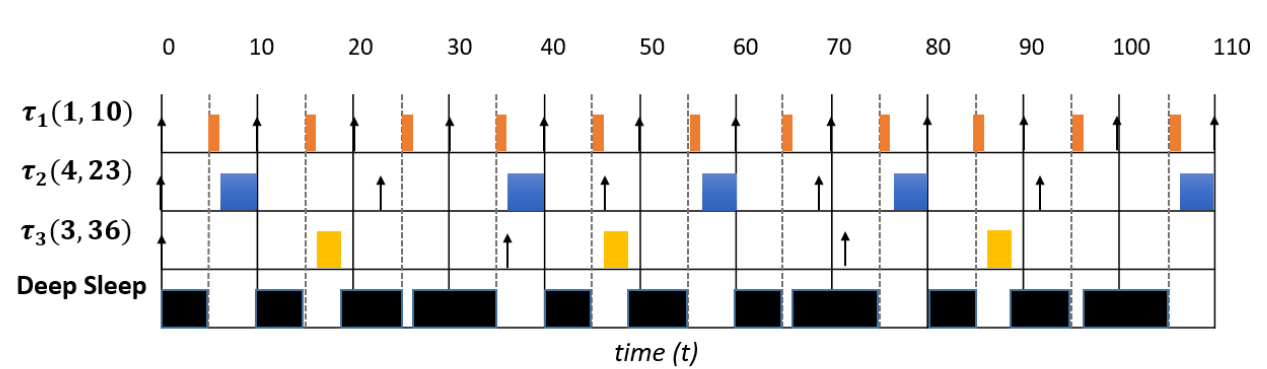
\includegraphics[height=4cm,width=12cm]{part1/rhs.png}
\captionof{figure}{Energy-Saving RHS}
\label{fig:exempleRHS}
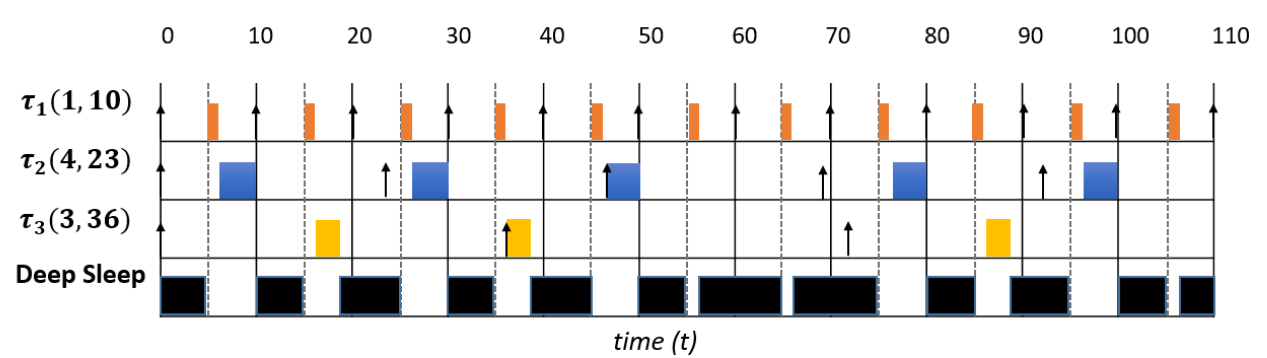
\includegraphics[height=4cm,width=12cm]{part1/rhs+.png}
\captionof{figure}{Energy-Saving RHS+}
\label{fig:exempleRHS+}
\end{center}

\section{Conclusion}

\part{Contributions}
\chapter{Endormissement de tache sous priorité Fixe}
\minitoc
\section{modéle de tâches}
Le modèle utilisé ici est le modèle de tâche périodique de Liu et
Layland défini au chapitre 1.\\ Soit $\taskset =
\{\task{1},\task{2},\cdots,\task{n}\}$ un ensemble de tache, chaque
tache $\task{i}$ est caracterisé par $\task{i} =
(\charge{i},\deadline{i},\period{i})$ et :
\begin{itemize}
\item $\task{i}$ est periodique.
\item $\charge{i}$ est le pire temps d'execution de la tache $i$.
\item $\deadline{i}$ est l'écheance relative de la tache $i$.
\item $\period{i}$ est la periode relative de la tache $i$.
\item l'ensemble de tâches $\taskset{}$ est ordonnançable avec
  l'algorithme Deadline Monotonic.
\end{itemize}
\section{Le cas monoprocesseur}
Dans cette section nous allons inserer une tâche d'endormissement
$\task{\sleep} = \{ \charge{\sleep}, \deadline{\sleep},
\period{\sleep}\}$ avec $\min \charge{\sleep} \leq \charge{\sleep}
\geq \max \charge{sleep}$ avec $\wcet{sleepMax} = (1-\util{}) \times
\period{H}$ et $\task{sleep} \cup \taskset{}$ est ordonnançable avec
Deadline Monotonic.


Pour cela nous presentons l'algorithme d'insertion de tache
d'endormissement $\task{\textsc{sleep}}$ dans un taskset $\taskset{}$.



\begin{algorithm}
\caption{Insertion Taches Endormissement Dans Un Mono-processeur}
\label{dmup}
\begin{algorithmic}
\State TaskSet $\taskset{}$, Temps Minimum d'execution $\wcetf_{SleepMin}$, Temps d'execution Maximum $\wcetf_{SleepMax}$, Pas de decrementation $\Delta \wcetf_{}$
\State Tache $\task{Sleep}$
\State $\wcetf_{Sleep}  \longleftarrow \wcetf_{SleepMax}$ 
\State $\deadline{Sleep}	\longleftarrow \period{H}$ 
\State $\period{sleep} \longleftarrow \period{H}$ 
\While {$\taskset{} \cup tache(\wcetf_{Sleep},\deadline{Sleep},\period{H})$ est non  ordonnançable et $\wcetf_{Sleep} \geq \wcetf_{SleepMin}$}
\State $\wcetf_{Sleep} \longleftarrow \wcetf_{Sleep} - \Delta \wcetf_{}$ 
\EndWhile 
\If {$\taskset{} \cup \task{sleep}$ est non ordonnançable \textbf{or} $\wcetf_{Sleep} \leq \wcetf_{SleepMin}$ \textbf{or} $!test(\task{sleep})$}
\State $\emptyset$
\EndIf
\State $\task{Sleep} \leftarrow Tache(\wcetf_{Sleep},\deadline{Sleep},\period{sleep})$
\end{algorithmic}
\end{algorithm}

Nous illustrons notre algorithme avec un
exemple d'application. Le tableau \ref{tab:exempledmup} et la figure
\ref{fig:exempledmupapr} represente un ensemble de tâches $\taskset{}$
ordonnançable par Deadline Monotonic où on a inseré une tache
d'endormissement $\task{\textsc{sleep}}$:

\begin{table}[!h]
\begin{center}
\begin{tabular}{|c|c|c|c|}
 \hline$\task{i}$ & $\charge{i}$ & $\deadline{i}$ & $\period{i}$ \\ 
 \hline 1 & 1 & 10 & 10 \\ 
 \hline 2 & 2 & 15 & 15 \\ 
 \hline 
 \end{tabular}
\end{center}
\caption{Ensemble de t\^aches periodiques} \label{tab:exempledmup}
\end{table}

%\begin{figure}[h]
%\begin{center}
%\begin{RTGrid}[height=4cm,width=12cm,labelsize=8pt,numbersize=6]{3}{31}
%\multido{\n=0+10}{3}{
%\TaskArrDead{1}{\n}{10}}
%\TaskArrDead{1}{20}{10}

%\TaskExecution{1}{3}{4}
%\TaskExecution{1}{13}{14}
%\TaskExecution{1}{23}{24}

%\multido{\n=0+15}{2}{
%\TaskArrDead{2}{\n}{15}}
%\TaskArrDead{2}{15}{15}
%\TaskExecution{2}{4}{5}
%\TaskExecution{2}{8}{9}
%\TaskExecution{2}{18}{20}

%\multido{\n=0+5}{6}{
%\TaskArrDead{3}{\n}{5}}
%\TaskArrDead{3}{25}{5}
%\TaskExecution{3}{0}{3}
%\TaskExecution{3}{5}{8}
%\TaskExecution{3}{10}{13}
%\TaskExecution{3}{15}{18}
%\TaskExecution{3}{20}{23}
%\TaskExecution{3}{25}{28}

%\end{RTGrid}
%\caption{Insertion de tache dans un monoprocesseur} \label{fig:exempledmup}
%\end{center}
%\end{figure}

\section{Le cas multiprocesseur}
Dans cette section nous allons inserer un ensemble de tâches
d'endormissement
$\{\task{\sleep}^1,\task{\sleep}^2,...,\task{\sleep}^m\}$ tel que
$\task{\sleep}^i = \{ \charge{\sleep}^i, \deadline{\sleep}^i,
\period{\sleep}^i\}$ dans m processeurs $\proc{} =
\{\proc{1},\proc{2},...,\proc{m}\}$.  \indent Pour cela nous
presentons nous presentons deux strategie d'insertion :

\begin{description}
\item{Insertion Locale :} Chaque processeur$_i$ à sa propre tache
  d'endormissement $\task{\sleep}^i$
\item{Insertion Globale :} Tous les processeur ont une même tache
  d'endormissement
  $\task{\sleep}=\task{\sleep}^1=\task{\sleep}^2=...=\task{\sleep}^m$
\end{description}
Les deux algorithmes representent l'inseretion locale (Resp. globale)
d'un ensemble de tâches d'endormissement dans un ensemble de
processeur.


\begin{algorithm}
\caption{Algorithme d'insertion de Tache d'endormissement en locale dans un multiprocesseur}
\label{dmmpl}
\begin{algorithmic}
\State Ensemble de processeur $\core{}$, Temps Minimum d'exécution $\wcetf_{SleepMin}$
\State Ensemble de Tache d'endormissement $\taskset{Sleep}$
\For{$ \proc{i} \in \core{}$}
\State $\task{sleep}^i$ = tache\_endormissement\_monoprocesseur($\wcetf_{SleepMin}$) 
\State $\taskset{Sleep}^i =\taskset{Sleep}^i \cup \task{sleep}^i$
\EndFor
\end{algorithmic}
\end{algorithm}

\begin{algorithm}
\caption{Algorithme d'insertion de Tache d'endormissement en globale dans un multiprocesseur}
\label{dmmpg}
\begin{algorithmic}
\State Ensemble de processeur $\core{}$, Temps Minimum d'exécution $\wcetf_{SleepMin}$
\State Ensemble de Tache d'endormissement $\taskset{Sleep}$
\State $\taskset{sleep} \leftarrow \emptyset$
\State $\task{sleep} \leftarrow \emptyset$
\State $\thrf \leftarrow PeriodeHarmonic(\taskset{Sleep})$
\For{$ \proc{i} \in \core{}$}
\State $\task{sleep}^i$ = tache\_endormissement\_monoprocesseur($\wcetf_{SleepMin},\thrf$) 
\State $\task{sleep} \leftarrow \task{sleep} \cup task{sleep}^i$
\EndFor
\For{$ \proc{i} \in \core{}$}
\State $\taskset{Sleep} \leftarrow \taskset{Sleep} \cup Min_{i =1..m}(\task{Sleep}^i)$
\EndFor
\end{algorithmic}
\end{algorithm}


Nous illustrons notre algorithme avec un exemple d'application. Le
tableau \ref{tab:exempledmmp} et les figures \ref{fig:exempledmmpl} et
\ref{fig:exempledmmpg} representent un ensemble de tâches $\taskset{}$
ordonnançable par Deadline Monotonic dans un multiprocesseur à 2
processeur en partitionnement FirstFit où on a inseré deux taches
d'endormissements $\task{\sleep}$ en locale et en globale.

\begin{figure}[!h]
\begin{center}
\begin{RTGrid}[width=10cm,nosymbols=1]{5}{31}
\RowLabel{3}{$\task{Sleep}$}
\TaskExecution[color=green]{3}{0}{4}
\TaskExecution[color=green]{3}{10}{14}
\TaskExecution[color=green]{3}{20}{24}
\RowLabel{1}{$\task{1}$}
\TaskExecution{1}{4}{9}
\TaskExecution{1}{14}{19}
\TaskExecution{1}{24}{29}
\RowLabel{2}{$\task{3}$}
\TaskExecution{2}{9}{10}
\TaskExecution{2}{19}{20}
\TaskExecution{2}{29}{30}
\RowLabel{4}{$\task{2}$}
\RowLabel{5}{$\task{Sleep}$}
\TaskExecution[color=green]{5}{0}{8}
\TaskExecution{4}{8}{15}
\TaskExecution[color=green]{5}{21}{28}
\TaskExecution{4}{28}{25}
\TaskNArrDead{1}{0}{10}{10}{3}
\TaskArrival{1}{30}
\TaskNArrDead{2}{0}{22}{24}{1}
\TaskArrival{2}{24}
\TaskNArrDead{3}{0}{10}{10}{3}
\TaskArrival{3}{30}
\TaskNArrDead{4}{0}{15}{21}{1}
\TaskArrival{4}{21}
\TaskNArrDead{5}{0}{15}{15}{2}
\TaskArrival{5}{30}
\end{RTGrid}
\end{center}
\caption{Insertion locale de tâches d'endormissements dans un multiprocesseur} \label{fig:dmmpl}
\end{figure}


\begin{figure}[!h]
\begin{center}
\begin{RTGrid}[width=10cm,nosymbols=1]{5}{31}

\RowLabel{3}{$\task{Sleep}$}
\RowLabel{1}{$\task{1}$}
\RowLabel{2}{$\task{3}$}
\RowLabel{4}{$\task{2}$}
\RowLabel{5}{$\task{Sleep}$}
\TaskNArrDead{1}{0}{10}{10}{3}
\TaskArrival{1}{30}
\TaskNArrDead{2}{0}{22}{24}{1}
\TaskArrival{2}{24}
\TaskNArrDead{3}{0}{5}{5}{6}
\TaskArrival{3}{30}
\TaskNArrDead{4}{0}{15}{21}{1}
\TaskArrival{4}{21}
\TaskNArrDead{5}{0}{5}{5}{6}
\TaskArrival{5}{30}



\TaskExecution[color=green]{3}{0}{4}
\TaskExecution[color=green]{3}{10}{14}
\TaskExecution[color=green]{3}{20}{24}


\TaskExecution{1}{4}{9}
\TaskExecution{1}{14}{19}
\TaskExecution{1}{24}{29}


\TaskExecution{2}{9}{10}
\TaskExecution{2}{19}{20}
\TaskExecution{2}{29}{30}

\TaskExecution[color=green]{5}{0}{4}
\TaskExecution[color=green]{5}{10}{14}
\TaskExecution[color=green]{5}{20}{24}

\TaskExecution{4}{4}{11}
\TaskExecution{4}{24}{30}

\end{RTGrid}
\end{center}
\caption{Insertion globale de tâches d'endormissements dans un multiprocesseur} \label{fig:dmmpg}
\end{figure}

\chapter{Endormissement de tache sous priorité dynamique}
\minitoc
\section{modéle de tâches}
Le modèle utilisé ici est le modèle de tâche sporadique.

Soit $\taskset{} = \{\task{1},\task{2},...,\task{n}\}$ un ensemble de
tache, chaque tache $\task{i}$ est caracterisé par $\task{i} =
(\charge{i},\deadline{i},\period{i})$ et :

\begin{itemize}
\item $\task{i}$ est sporadique.
\item $\charge{i}$ est le pire temps d'execution de la t\^ache $i$
\item $\deadline{i}$ est l'écheance relative de la t\^ache $i$
\item $\period{i}$ est la periode de la t\^ache $i$
\item l'ensemble de tâches $\taskset{}$ est ordonnançable avec l'algorithme EarliestDeadlineFirst
\end{itemize}

\section{Limitation de nombre de preemption}

%\begin{center}
%\begin{algorithm}[H]
%\KwData{TaskSet de tâches sporadic $\taskset{}$}
%\KwResult{$Q(t)$}
%\Begin{
% Posons $\{t_{1},t_{2},...,t_{n}\}$ ensemble ordonné de $\{\deadline{i}+l\periode{i},\forall l \in N, 1 \leq i \leq n \}$ où $(t_{k} < t_{k+1},\forall k)$
% $Q(t_{1}) \leftarrow t_{1} - \sum_{\tache{i} \in \taskset{}} DBF(\tache{i},t_{1})$\;
% \For{$k \leftarrow 2,3...$}{
%	$Q(t_{k}) \leftarrow Min(Q(t_{k-1}),t_{k} - \sum_{\tache{i} \in \taskset{}} DBF(\tache{i},t_{k}))$\;
%	\If{$Q(t_{k}) < 0$}{
%	\textbf{return} faux\;
%	}
%	}
%	\textbf{return} vrai\;
% }
%\caption{Insertion Taches Endormissement Dans Un Mono-processeur}
%\end{algorithm}
%\end{center}

\section{Le cas monoprocesseur}
%\begin{center}
\begin{algorithm}[H]
\KwData{TaskSet $\taskset{}$, Temps Minimum d'execution $\wcet{SleepMin}$, Temps d'execution Maximum $\wcet{SleepMax}$, Pas de decrementation $\Delta \wcet{}$}
\KwResult{Tache $\tache{Sleep}$}
\Begin{
 $\wcet{Sleep}  \longleftarrow \wcet{SleepMax}$ \;
 $\deadline{Sleep}	\longleftarrow \periode{H}$ \;
 $\periode{sleep} \longleftarrow \periode{H}$ \;
 \While{$\Gamma \cup tache(\wcet{Sleep},\deadline{Sleep},\periode{H})$ est non  ordonnançable et $\wcet{Sleep} \geq \wcet{SleepMin}$}
 {
 	$\wcet{Sleep} \longleftarrow \wcet{Sleep} - \Delta \wcet{}$ \;
 }
 $\tache{Sleep} \longleftarrow CreerTache(\wcet{Sleep},\deadline{Sleep},\periode{sleep})$
 }
 \caption{Insertion Taches Endormissement Dans Un Mono-processeur}
\end{algorithm}
\end{center}

\begin{table}[!h]
\begin{center}
\begin{tabular}{|c|c|c|c|}
 \hline$\task{i}$ & $\charge{i}$ & $\deadline{i}$ & $\period{i}$ \\ 
 \hline 1 & 2 & 25 & 25 \\ 
 \hline 2 & 2 & 10 & 10 \\ 
 \hline 
 \end{tabular}
\end{center}
\caption{Ensemble de taches periodiques} \label{tab:exempleedfmp}
\end{table}

%\begin{figure}[h]
%\begin{center}
%\begin{RTGrid}[height=4cm,width=12cm,labelsize=8pt,numbersize=6]{3}{32}

%\multido{\n=0+25}{1}{
%\TaskArrDead{1}{\n}{25}}
%\TaskArrDead{1}{20}{10}

%\TaskExecution{1}{9}{10}
%\TaskExecution{1}{19}{20}
%\TaskExecution{1}{29}{30}

%\multido{\n=0+10}{3}{
%\TaskArrDead{2}{\n}{10}}
%\TaskArrDead{2}{15}{15}
%\TaskExecution{2}{0}{2}
%\TaskExecution{2}{10}{12}
%\TaskExecution{2}{20}{22}
%\TaskExecution{2}{30}{32}

%\multido{\n=0+10}{3}{
%\TaskArrDead{3}{\n}{10}}
%%\TaskArrDead{3}{25}{5}
%\TaskExecution{3}{2}{9}
%\TaskExecution{3}{12}{19}
%\TaskExecution{3}{22}{29}

%\end{RTGrid}
%\caption{Insertion de tache dans un monoprocesseur} \label{fig:exempleedfmp}
%\end{center}
%\end{figure}

\section{Le cas multiprocesseur}

%Réécris les algorithmes ici !! et pas dans un autre fichier en utilisant le package algorithmic !
%\begin{center}
\begin{algorithm}[H]
\KwData{Ensemble de processeur $\proc{}$, Temps Minimum d'execution $\wcet{SleepMin}$}
\KwResult{Ensemble de Tache d'endormissement $\taskset{Sleep}$}
\Begin{
	\For{$ \proc{i} \in \proc{}$}
	{
		$\tache{sleep}^i$ = tache\_endormissement\_monoprocesseur($\wcet{SleepMin}$) \; 
		$\taskset{Sleep}^i =\taskset{Sleep}^i \cup \tache{sleep}^i$
		}
	}
 \caption{Insertion Globale de Taches Endormissement Dans Une architecture Multiprocesseur}
\end{algorithm}
\end{center}
%\begin{center}
\begin{algorithm}[H]
\KwData{Ensemble de processeur $\proc{}$, Temps Minimum d'execution $\wcet{SleepMin}$}
\KwResult{Ensemble de Tache d'endormissement $\taskset{Sleep}$}
\Begin{
	$\tache{sleep} \rightarrow \emptyset$ \;
	\For{$ \proc{i} \in \proc{}$}
	{
		$\tache{sleep}^i$ = tache\_endormissement\_monoprocesseur($\wcet{SleepMin}$) \; 
		$\tache{sleep} \rightarrow \tache{sleep} \cup \tache{sleep}^i$
	}
	\For{$ \proc{i} \in \proc{}$}
	{
		$\taskset{sleep}^i \rightarrow \taskset{sleep}^i \cup Min_{i =1..m}(\tache{sleep}^i)$
	}
	}
 \caption{Insertion Globale de Taches Endormissement Dans Une architecture Multiprocesseur}
\end{algorithm}
\end{center}

\begin{table}[h]
\begin{center}
\begin{tabular}{|c|c|c|c|}
 \hline$\task{i}$ & $\charge{i}$ & $\deadline{i}$ & $\period{i}$ \\ 
 \hline1 & 2 & 10 & 10 \\ 
 \hline 2 & 2 & 15 & 21 \\ 
 \hline 
 \end{tabular}
\end{center}
\caption{Insertion locale de tâches d'endormissements dans un multiprocesseur} \label{tab:edfmp}
\end{table}
\section{insertion locale}
\begin{figure}[!h]
\begin{center}
\resizebox{15cm}{4cm}{
\begin{tikzpicture}
\node at (-0.5,0.5) {P1};
\node at (-0.5,1.5) {P2};
%P1
\draw[fill=white] (0.0,0) rectangle (12,1) ;

\draw[fill=red] (0.0,0) rectangle (0.3,1) ;
\draw[fill=blue] (0.3,0) rectangle (0.5,1) ;

\draw[fill=red] (1.0,0) rectangle (1.3,1) ;
\draw[fill=blue] (1.3,0) rectangle (1.5,1) ;

\draw[fill=red] (2.0,0) rectangle (2.3,1) ;
\draw[fill=blue] (2.3,0) rectangle (2.5,1) ;

\draw[fill=red] (3.0,0) rectangle (3.3,1) ;
\draw[fill=blue] (3.3,0) rectangle (3.5,1) ;

\draw[fill=red] (4.0,0) rectangle (4.3,1) ;
\draw[fill=blue] (4.3,0) rectangle (4.5,1) ;

\draw[fill=red] (5.0,0) rectangle (5.3,1) ;
\draw[fill=blue] (5.3,0) rectangle (5.5,1) ;

\draw[fill=red] (6.0,0) rectangle (6.3,1) ;
\draw[fill=blue] (6.3,0) rectangle (6.5,1) ;

\draw[fill=red] (7.0,0) rectangle (7.3,1) ;
\draw[fill=blue] (7.3,0) rectangle (7.5,1) ;

\draw[fill=red] (8.0,0) rectangle (8.3,1) ;
\draw[fill=blue] (8.3,0) rectangle (8.5,1) ;

\draw[fill=red] (9.0,0) rectangle (9.3,1) ;
\draw[fill=blue] (9.3,0) rectangle (9.5,1) ;

\draw[fill=red] (10.0,0) rectangle (10.3,1) ;
\draw[fill=blue] (10.3,0) rectangle (10.5,1) ;

\draw[fill=red] (11.0,0) rectangle (11.3,1) ;
\draw[fill=blue] (11.3,0) rectangle (11.5,1) ;
%P2
\draw[fill=white] (0.0,1) rectangle (12,2) ;

\draw[fill=yellow] (0.0,1) rectangle (0.2,2) ;
\draw[fill=red] (0.2,1) rectangle (1.1,2) ;

\draw[fill=yellow] (2.1,1) rectangle (2.2999999046325685,2) ;
\draw[fill=red] (2.2999999046325685,1) rectangle (3.1999999046325684,2) ;

\draw[fill=yellow] (4.2,1) rectangle (4.399999809265137,2) ;
\draw[fill=red] (4.399999809265137,1) rectangle (5.299999809265136,2) ;

\draw[fill=yellow] (6.2999997,1) rectangle (6.499999713897705,2) ;
\draw[fill=red] (6.499999713897705,1) rectangle (7.399999713897705,2) ;

\draw[fill=yellow] (8.4,1) rectangle (8.599999618530273,2) ;
\draw[fill=red] (8.599999618530273,1) rectangle (9.499999618530273,2) ;

\draw[fill=yellow] (10.5,1) rectangle (10.7,2) ;
\draw[fill=red] (10.7,1) rectangle (11.6,2) ;
%%%%%%%
\draw [->](0,-1) -- coordinate (x axis mid) (12.5,-1);
\draw (0,-1) -- (0,-1.5) node[fill=white,rotate=90] {0};
\draw (1,-1) -- (1,-1.5) node[fill=white,rotate=90] {10};
\draw (2,-1) -- (2,-1.5) node[fill=white,rotate=90] {20};
\draw (3,-1) -- (3,-1.5) node[fill=white,rotate=90] {30};
\draw (4,-1) -- (4,-1.5) node[fill=white,rotate=90] {40};
\draw (5,-1) -- (5,-1.5) node[fill=white,rotate=90] {50};
\draw (6,-1) -- (6,-1.5) node[fill=white,rotate=90] {60};
\draw (7,-1) -- (7,-1.5) node[fill=white,rotate=90] {70};
\draw (8,-1) -- (8,-1.5) node[fill=white,rotate=90] {80};
\draw (9,-1) -- (9,-1.5) node[fill=white,rotate=90] {90};
\draw (10,-1) -- (10,-1.5) node[fill=white,rotate=90] {100};
\draw (11,-1) -- (11,-1.5) node[fill=white,rotate=90] {110};
\draw (12,-1) -- (12,-1.5) node[fill=white,rotate=90] {120};

\draw[fill=white] (12.2,-0.4) rectangle (15.5,2.2) ;
\draw[fill=red] (12.6,0) rectangle (13.2,0.2) ;
\draw (14.5,0) -- (14.5,0) node[fill=white] {DeepSleep};
\draw[fill=blue] (12.6,0.5) rectangle (13.2,0.7) ;
\draw (14.5,0.5) -- (14.5,0.5) node[fill=white] {$\tau_1$};
\draw[fill=yellow] (12.6,1) rectangle (13.2,1.2) ;
\draw (14.5,1) -- (14.5,1) node[fill=white] {$\tau_2$};
\end{tikzpicture}}
\end{center}
\caption{Insertion globale de tâches d'endormissements dans un multiprocesseur} \label{fig:edfmpl}
\end{figure}
\section{insertion globale}
\begin{figure}[!h]
\begin{center}
\resizebox{15cm}{4cm}{
\begin{tikzpicture}
\node at (-0.5,0.5) {P1};
\node at (-0.5,1.5) {P2};
%P1
\draw[fill=white] (0.0,0) rectangle (12,1) ;

\draw[fill=red] (0.0,0) rectangle (0.3,1) ;
\draw[fill=blue] (0.3,0) rectangle (0.5,1) ;

\draw[fill=red] (1.0,0) rectangle (1.3,1) ;
\draw[fill=blue] (1.3,0) rectangle (1.5,1) ;

\draw[fill=red] (2.0,0) rectangle (2.3,1) ;
\draw[fill=blue] (2.3,0) rectangle (2.5,1) ;

\draw[fill=red] (3.0,0) rectangle (3.3,1) ;
\draw[fill=blue] (3.3,0) rectangle (3.5,1) ;

\draw[fill=red] (4.0,0) rectangle (4.3,1) ;
\draw[fill=blue] (4.3,0) rectangle (4.5,1) ;

\draw[fill=red] (5.0,0) rectangle (5.3,1) ;
\draw[fill=blue] (5.3,0) rectangle (5.5,1) ;

\draw[fill=red] (6.0,0) rectangle (6.3,1) ;
\draw[fill=blue] (6.3,0) rectangle (6.5,1) ;

\draw[fill=red] (7.0,0) rectangle (7.3,1) ;
\draw[fill=blue] (7.3,0) rectangle (7.5,1) ;

\draw[fill=red] (8.0,0) rectangle (8.3,1) ;
\draw[fill=blue] (8.3,0) rectangle (8.5,1) ;

\draw[fill=red] (9.0,0) rectangle (9.3,1) ;
\draw[fill=blue] (9.3,0) rectangle (9.5,1) ;

\draw[fill=red] (10.0,0) rectangle (10.3,1) ;
\draw[fill=blue] (10.3,0) rectangle (10.5,1) ;

\draw[fill=red] (11.0,0) rectangle (11.3,1) ;
\draw[fill=blue] (11.3,0) rectangle (11.5,1) ;
%P2
\draw[fill=white] (0.0,1) rectangle (12,2) ;

\draw[fill=red] (0.0,1) rectangle (0.3,2) ;
\draw[fill=red] (1.0,1) rectangle (1.3,2) ;
\draw[fill=red] (2.0,1) rectangle (2.3,2) ;
\draw[fill=red] (3.0,1) rectangle (3.3,2) ;
\draw[fill=red] (4.0,1) rectangle (4.3,2) ;
\draw[fill=red] (5.0,1) rectangle (5.3,2) ;
\draw[fill=red] (6.0,1) rectangle (6.3,2) ;
\draw[fill=red] (7.0,1) rectangle (7.3,2) ;
\draw[fill=red] (8.0,1) rectangle (8.3,2) ;
\draw[fill=red] (9.0,1) rectangle (9.3,2) ;
\draw[fill=red] (10.0,1) rectangle (10.3,2) ;
\draw[fill=red] (11.0,1) rectangle (11.3,2) ;

\draw[fill=yellow] (0.3,1) rectangle (0.5,2) ;
\draw[fill=yellow] (2.3,1) rectangle (2.5,2) ;
\draw[fill=yellow] (4.3,1) rectangle (4.5,2) ;
\draw[fill=yellow] (6.3,1) rectangle (6.5,2) ;
\draw[fill=yellow] (8.4,1) rectangle (8.6,2) ;
\draw[fill=yellow] (10.5,1) rectangle (10.7,2) ;
%%%%%%%
\draw [->](0,-1) -- coordinate (x axis mid) (12.5,-1);
\draw (0,-1) -- (0,-1.5) node[fill=white,rotate=90] {0};
\draw (1,-1) -- (1,-1.5) node[fill=white,rotate=90] {10};
\draw (2,-1) -- (2,-1.5) node[fill=white,rotate=90] {20};
\draw (3,-1) -- (3,-1.5) node[fill=white,rotate=90] {30};
\draw (4,-1) -- (4,-1.5) node[fill=white,rotate=90] {40};
\draw (5,-1) -- (5,-1.5) node[fill=white,rotate=90] {50};
\draw (6,-1) -- (6,-1.5) node[fill=white,rotate=90] {60};
\draw (7,-1) -- (7,-1.5) node[fill=white,rotate=90] {70};
\draw (8,-1) -- (8,-1.5) node[fill=white,rotate=90] {80};
\draw (9,-1) -- (9,-1.5) node[fill=white,rotate=90] {90};
\draw (10,-1) -- (10,-1.5) node[fill=white,rotate=90] {100};
\draw (11,-1) -- (11,-1.5) node[fill=white,rotate=90] {110};
\draw (12,-1) -- (12,-1.5) node[fill=white,rotate=90] {120};

\draw[fill=white] (12.2,-0.4) rectangle (15.5,2.2) ;
\draw[fill=red] (12.6,0) rectangle (13.2,0.2) ;
\draw (14.5,0) -- (14.5,0) node[fill=white] {DeepSleep};
\draw[fill=blue] (12.6,0.5) rectangle (13.2,0.7) ;
\draw (14.5,0.5) -- (14.5,0.5) node[fill=white] {$\tau_1$};
\draw[fill=yellow] (12.6,1) rectangle (13.2,1.2) ;
\draw (14.5,1) -- (14.5,1) node[fill=white] {$\tau_2$};
\end{tikzpicture}}
\end{center}
\caption{} \label{fig:edfmpg}
\end{figure}


\chapter{Expérimentations}
\section{La génération des taches}
\subsection{Cas monoprocesseur}
\subsubsection{Algorithmes UUnifast}
L’algorithme UUnifast \cite{} est un algorithme mis au point pour la
génération de taux d’utilisation sur monoprocesseur. Il génère une
distribution uniforme de n taux d’utilisation non biaisés à partir du
nombre de tâches n de l’ensemble et du taux d’utilisation processeur
total souhaité U.  UUnifast est un algorithme efficace de complexité
O(n). Nous rappelons qu’un ensemble au taux d’utilisation supérieur à
1 est trivialement non ordonnançable puisque l’utilisation processeur
dépasse alors le temps maximal disponible.
\subsubsection{Génération des périodes}
Lors de la génération de tâches, le choix des périodes est un élément
sensible pour les tests d’ordonnançabilité. En effet, certains de ces
tests basent leur analyse sur un intervalle de faisabilité.  La
longueur de cet intervalle dépend du plus petit commun multiple des
périodes (ppcm) appelée l’hyper-période. Si les périodes sont grandes,
premières entre elles, l’hyperpériode explose. Le défi consiste donc à
générer des périodes aléatoirement tout en limitant la taille de
l’hyper-période et c’est l’objet de la méthode de Goossens et Macq
\cite{Goossens01}.
\subsubsection{Génération des échéances}
Similairement à Goossens et Macq dans \cite{Goossens01}, nous generons
les échéances des taches generées. Nous déterminons aléatoirement
l’échéance dans un intervalle [$0.75 \times T_i$, $T_i$].  En résumé,
$Di = \lbrace T_i \times C_i) \times aleatoire(0.75 \times T_i,
T_i)\rbrace + C_i$ avec aleatoire(dmin, dmax) retourne un nombre réel
pseudo-aléatoire uniformément distribué sur l’intervalle [dmin, dmax]
et où la fonction arrondi(x) retourne l’entier le plus proche de x.
\subsection{Cas multiprocesseur}
\subsubsection{Algorithme UUnifast-Discard}
La méthode UUnifast présentée dans le cas monoprocesseur n’est pas
utilisée en contexte multiprocesseur, lorsque le taux d’utilisation du
processeur U peut dépasser 1. En effet, lorsque que le taux
d’utilisation total dépasse 1, UUnifast présente le risque de générer
des taux d’utilisation par tâche supérieurs à 1. Tâche qu’il n’est
alors possible d’ordonnancer sur aucun processeur.  Pour y remédier,
Davis et Burns \cite{DB11} ont proposé une extension appelée
UUnifast-Discard. Elle consiste simplement à employer UUnifast avec U
supérieur à 1 et à rejeter les ensembles pour lesquelles au moins un
taux d’utilisation par tâche est supérieur à 1. Son implantation est
simple mais cette méthode a l’inconvénient d’être particulièrement
inefficace lorsque U approche $\frac{n}{2}$ \cite{Emb10}.
\section{La simulation}
\section{Discussions}

\printbibliography[heading=bibintoc]
\end{document}
